\subsection{IFIT Subcellular Localisation During Interferon Induction and RSV Infection} \label{subsec:IFIT Subcellular Localisation During Interferon INduction and RSV Infection}
put antibody validation wbs

compare and contrast to the info in databases and papers

% introduction to ib stuff from my study
write about ib size statistics from my analysis

\begin{figure}
    \centering
    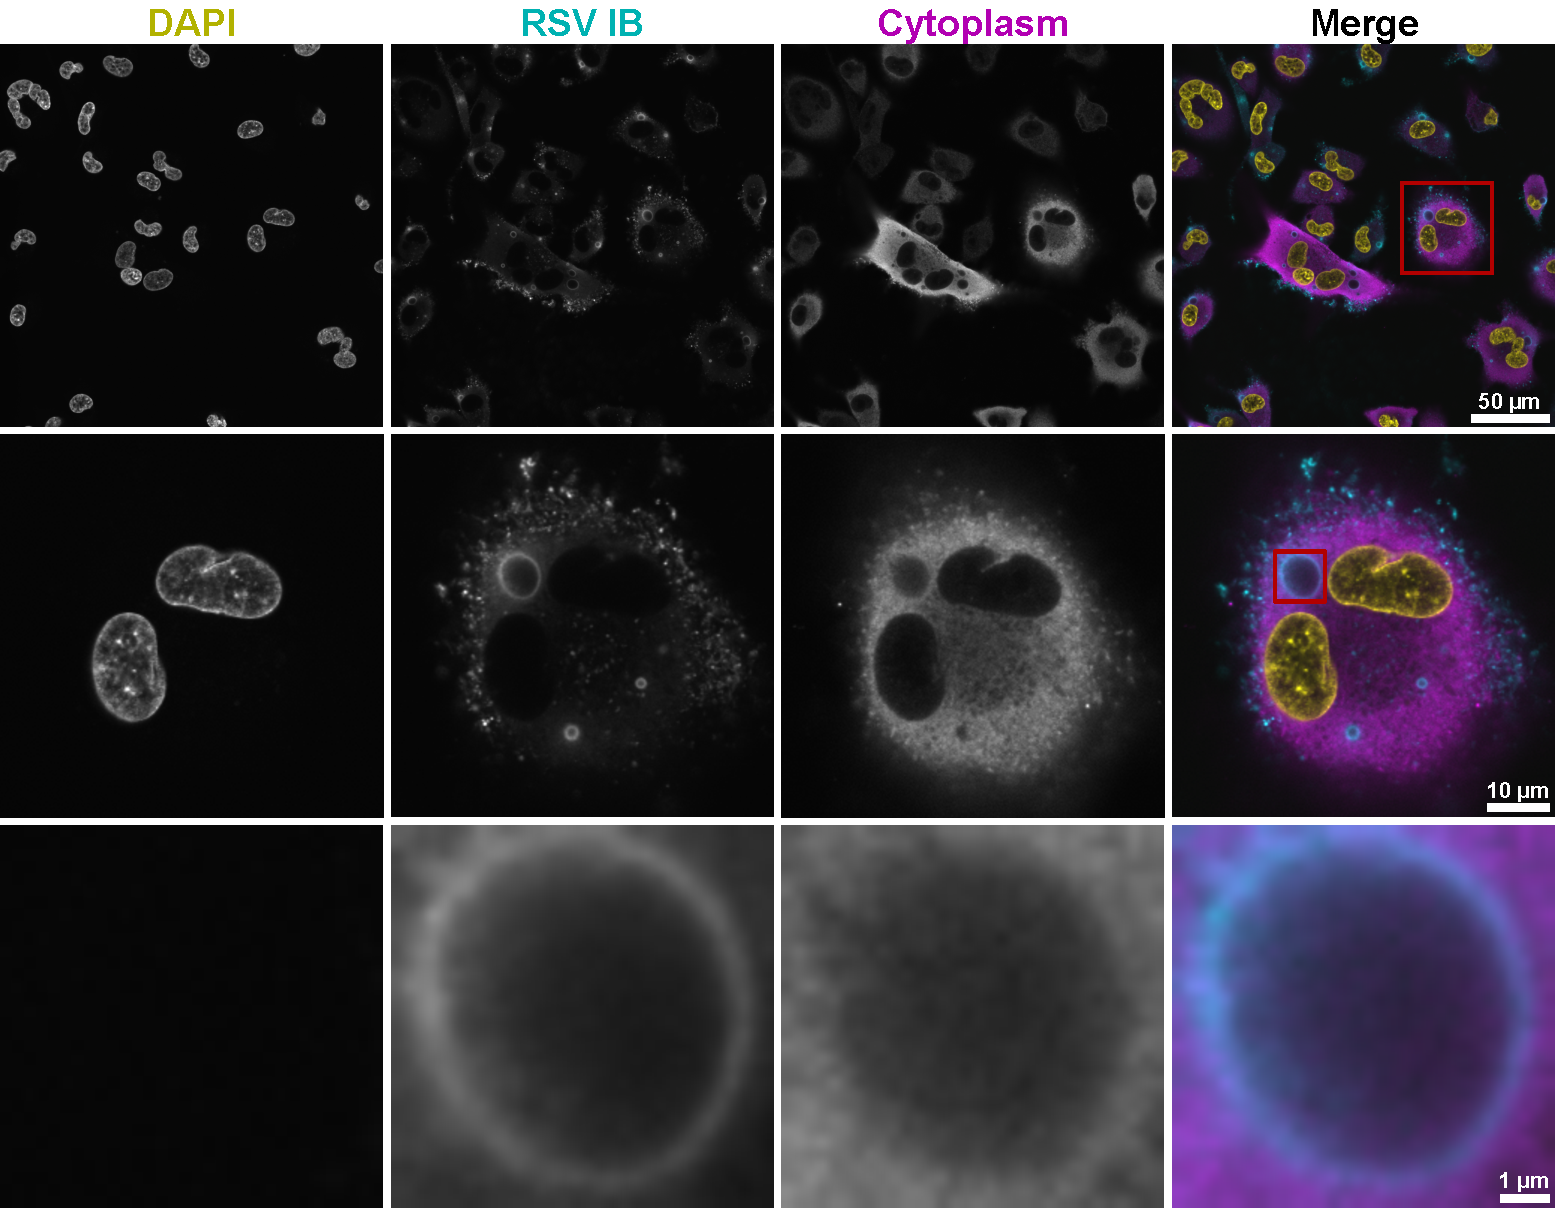
\includegraphics[width=1\linewidth]{09. Chapter 4/Figs/01. Localisation introduction/01. IB-zooms.pdf}
    \caption[Inclusion Bodies Within RSV Infected Cells: Zoom Sequence.]{\textbf{Inclusion Bodies Within RSV Infected Cells: Zoom Sequence.} A represerenative image of RSV infected cells detected using confocal microscopy. Cellular nuclei were stained with DAPI and are shown in yellow; RSV inclusion bodies are shown in cyan; and the cytoplasm is shown in magenta. Figure highlights a zoom sequence from a population of cells, into a single syncytia view, with lastly focusing at one individual inclusion body.}
    \label{fig:Inclusion Bodies Within RSV Infected Cells: Zoom Sequence}
\end{figure}


\begin{figure}
    \begin{subfigure}{0.495\textwidth}
        \caption{}
        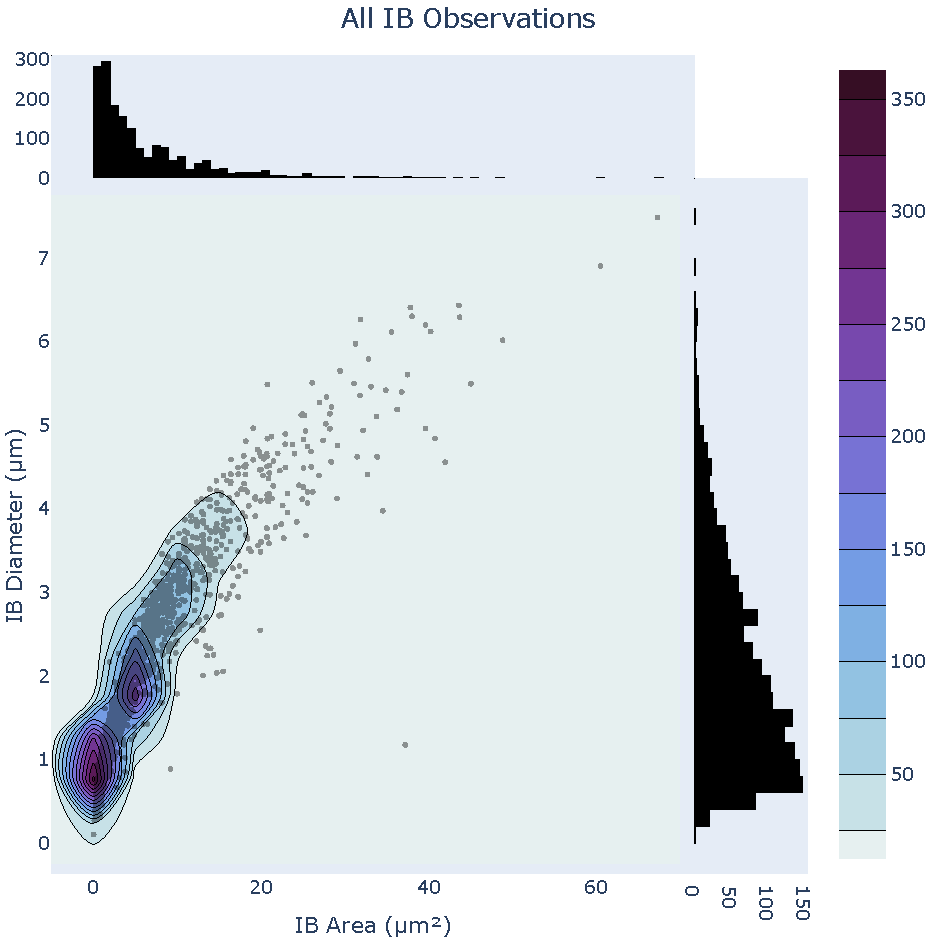
\includegraphics[width=\textwidth]{09. Chapter 4/Figs/01. Localisation introduction/02. heatmap_all.pdf} 
    \end{subfigure}
    \hfill
    \begin{subfigure}{0.495\textwidth}
        \caption{}
        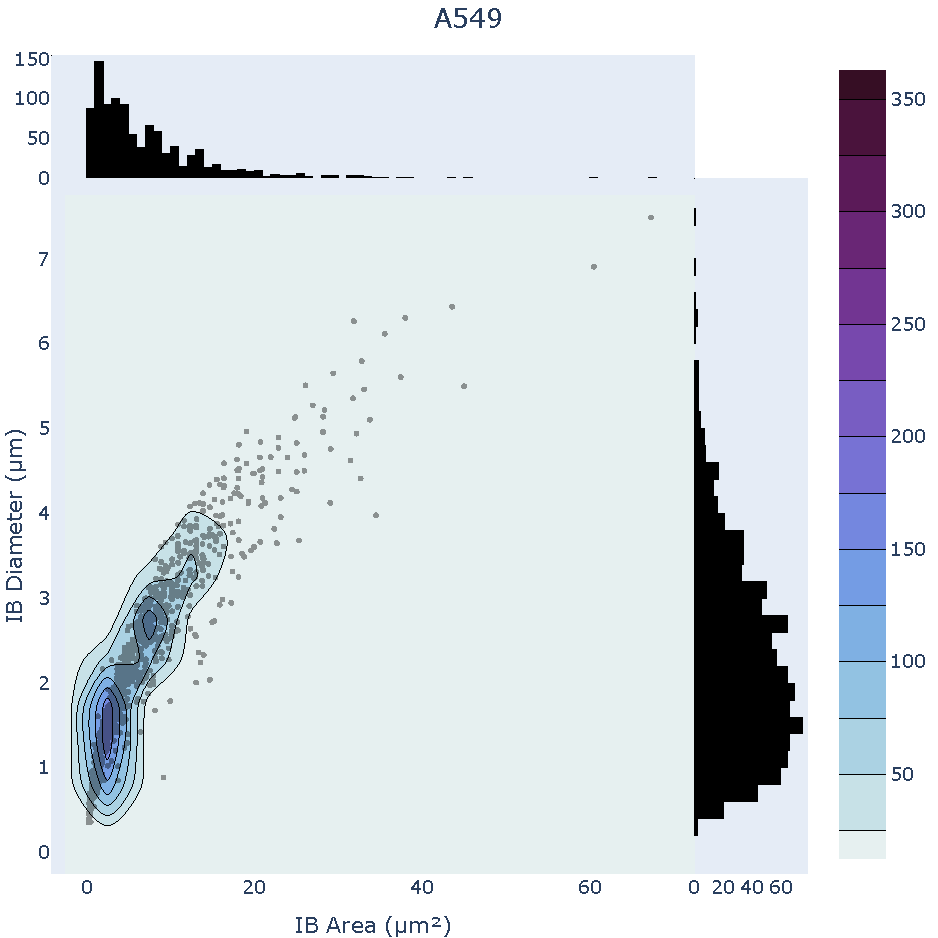
\includegraphics[width=\textwidth]{09. Chapter 4/Figs/01. Localisation introduction/03. heatmap_a549.pdf}
    \end{subfigure}

    \medskip
    \begin{subfigure}{0.495\textwidth}
        \caption{}
        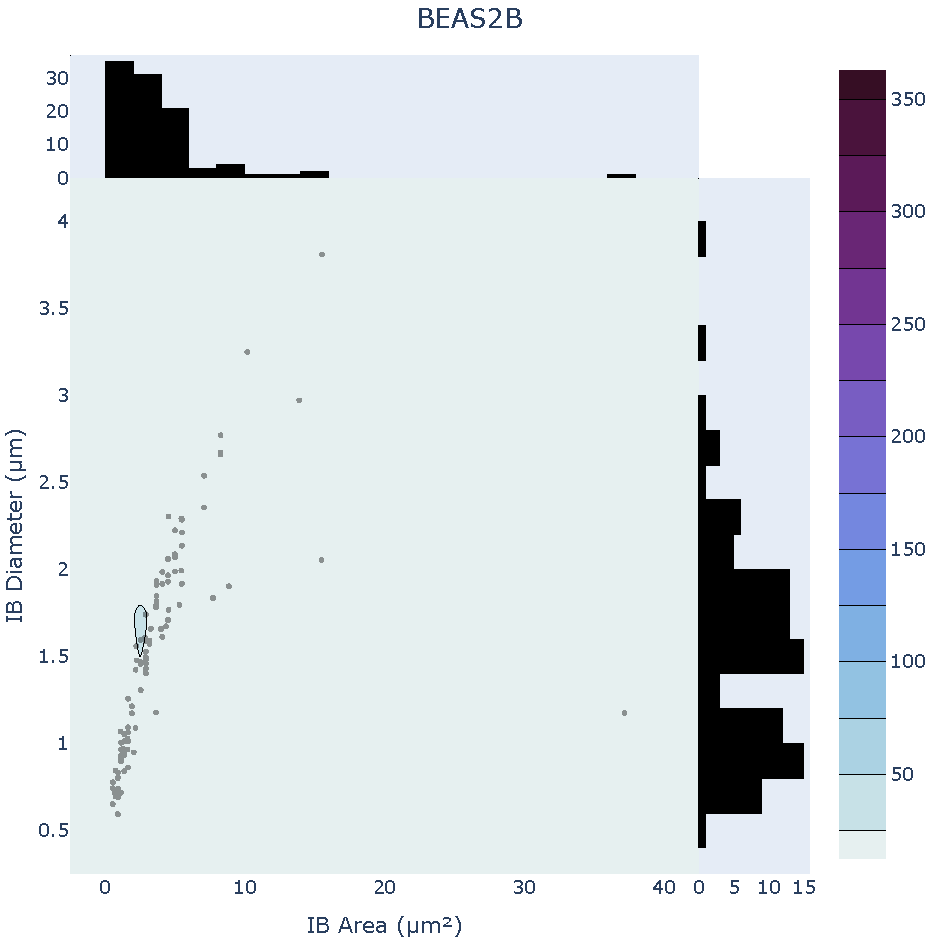
\includegraphics[width=\textwidth]{09. Chapter 4/Figs/01. Localisation introduction/04. heatmap_beas2b.pdf} 
    \end{subfigure}
    \hfill
    \begin{subfigure}{0.495\textwidth}
        \caption{}
        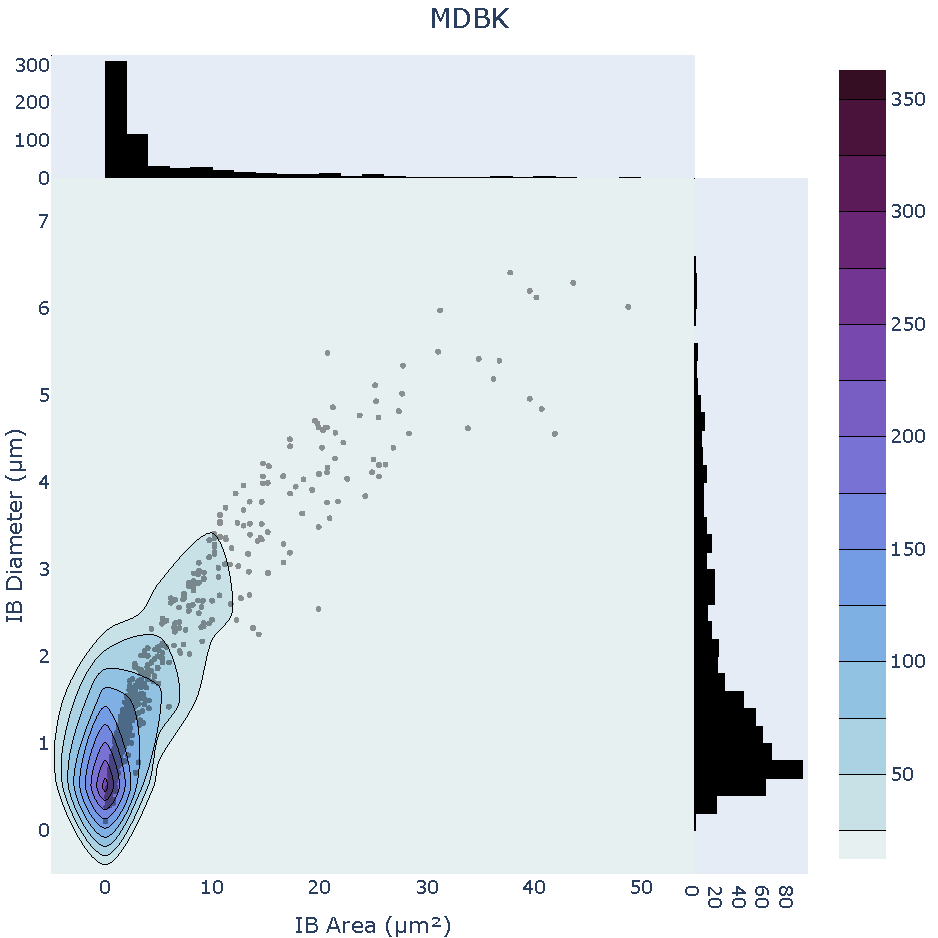
\includegraphics[width=\textwidth]{09. Chapter 4/Figs/01. Localisation introduction/05. heatmap_mdbk.pdf} 
    \end{subfigure}
    
    \caption[Size Characterization of Inclusion Bodies Across Different Cell Lines.]{\textbf{Size Characterization of Inclusion Bodies Across Different Cell Lines.} This figure presents the relationship between the measured area (\(\mu m^2\)) and diameter (\(\mu m\)) of individual inclusion bodies (IBs) as observed within the scope of this study. Additionally, the figure includes distinct population distributions depicted alongside the plots, representing (a) the aggregate of 1727 observations of IBs across all individual cell lines, (b) 1008 observations from the A549 cell line, (c) 99 observations from the BEAS2B cell line, and (d) 620 observations from the MDBK cell line. Contour plots are incorporated to elucidate the underlying density of individual IBs within the plots.}
    \label{fig:Size Characterization of Inclusion Bodies Across Different Cell Lines}
    
\end{figure}


% human stuff
Asdfasfsdfasdf \newline
IF Mock | INF | Infection \newline
A549 BEAS2B

Merge pictures of clusters of cells looking at changes between subcellular localisation and a clear increase in mean intensity. Graphs show mean intensity changes from all cells imaged.

\begin{figure}
    \centering
    \vspace{-15.74707pt}
    \includegraphics[width=1\linewidth]{09. Chapter 4/Figs/01. Localisation introduction/06. a549 merges.pdf}
    \caption[The Changes in Subcellular Localisation of Human IFITs in A549 Cells Subjected to hIFN\(\alpha\) or hRSV.]{\textbf{The Changes in Subcellular Localisation of Human IFITs in A549 Cells Subjected to hIFN\(\alpha\) or hRSV.} A549 cell were either mock treated, or treated with 1000 IU/mL of hIFN\(\alpha\) for 24 hours, or were infected with hRSV MOI 1 for 24 hours. Cells were fixed, and stained with DAPI (nuclei detection; yellow), anti-RSV N antibody (cyan), or with antibodies against IFIT proteins (magenta). Two antibodies against IFIT2 were used, termed IFIT2A and IFIT2B. Insets with magnified selections were created from infected images to more easily convey the underlying subcellular localisations.}
    \label{fig:The Changes in Subcellular Localisation of Human IFITs in A549 Cells Subjected to hIFN\(\alpha\) or hRSV.}
\end{figure}

\begin{figure}
    \centering
    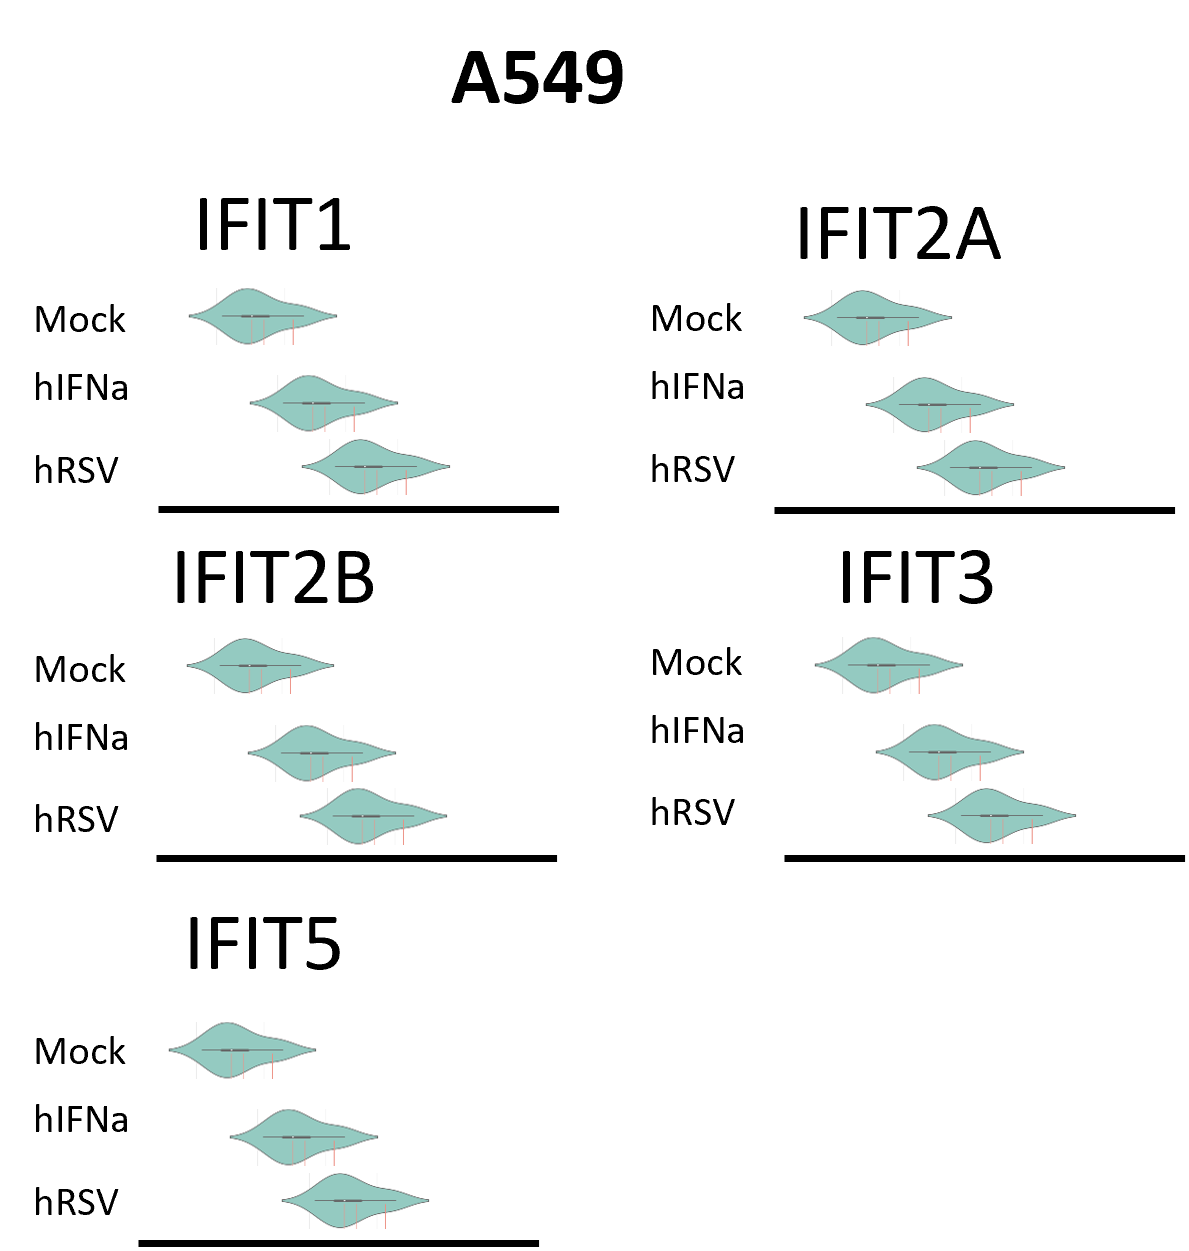
\includegraphics[width=1\linewidth]{09. Chapter 4/Figs/01. Localisation introduction/07. a549 plots.png}
    \caption[Quantification Of Expression Changes of Human IFITs in A549 Cells Subjected to hIFN\(\alpha\) or hRSV.]{\textbf{Quantification Of Expression Changes of Human IFITs in A549 Cells Subjected to hIFN\(\alpha\) or hRSV.} Nascent bovine IFIT1 in the context of bRSV infection has been observed to localise with the respect of IB in three distinct spaces. We observed it either concentrated inside the central point of the IB structure, while having reduced signal on the inner IB edge, compared to the cytoplasm (top and bottom panels), being excluded from the IB structure (3rd panel), or colocalising on the inner edge of the IB structure while having reduced signal in the middle of the structure compared to cytoplasm, or the edge staining (2nd panel).}
    \label{fig:Quantification Of Expression Changes of Human IFITs in A549 Cells Subjected to hIFNa or hRSV.}
\end{figure}


% bovine stuff
Asdfasfsdfasdf \newline
IF Mock | INF | Infection \newline
MDBK BT

Merge pictures of clusters of cells looking at changes between subcellular localisation and a clear increase in mean intensity. Graphs show mean intensity changes from all cells imaged.

\begin{figure}
    \centering
    \vspace{-15.74707pt}
    \includegraphics[width=1\linewidth]{09. Chapter 4/Figs/01. Localisation introduction/08. mdbk-merges-test.pdf}
    \caption[The Changes in Subcellular Localisation of Bovine IFITs in MDBK Cells Subjected to bIFN\(\alpha\) or bRSV.]{\textbf{The Changes in Subcellular Localisation of Bovine IFITs in MDBK Cells Subjected to bIFN\(\alpha\) or bRSV.} MDBK cell were either mock treated, or treated with 5 ng/mL of bIFN\(\alpha\) for 24 hours, or were infected with bRSV MOI 1 for 24 hours. Cells were fixed, and stained with DAPI (nuclei detection; yellow), anti-RSV N antibody (cyan), or with antibodies against IFIT proteins (magenta). Two antibodies against IFIT2 were used, termed IFIT2A and IFIT2B. Insets with magnified selections were created from infected images to more easily convey the underlying subcellular localisations.}
    \label{fig:The Changes in Subcellular Localisation of Bovine IFITs in MDBK Cells Subjected to bIFNa or bRSV}
\end{figure}

\begin{figure}
    \centering
    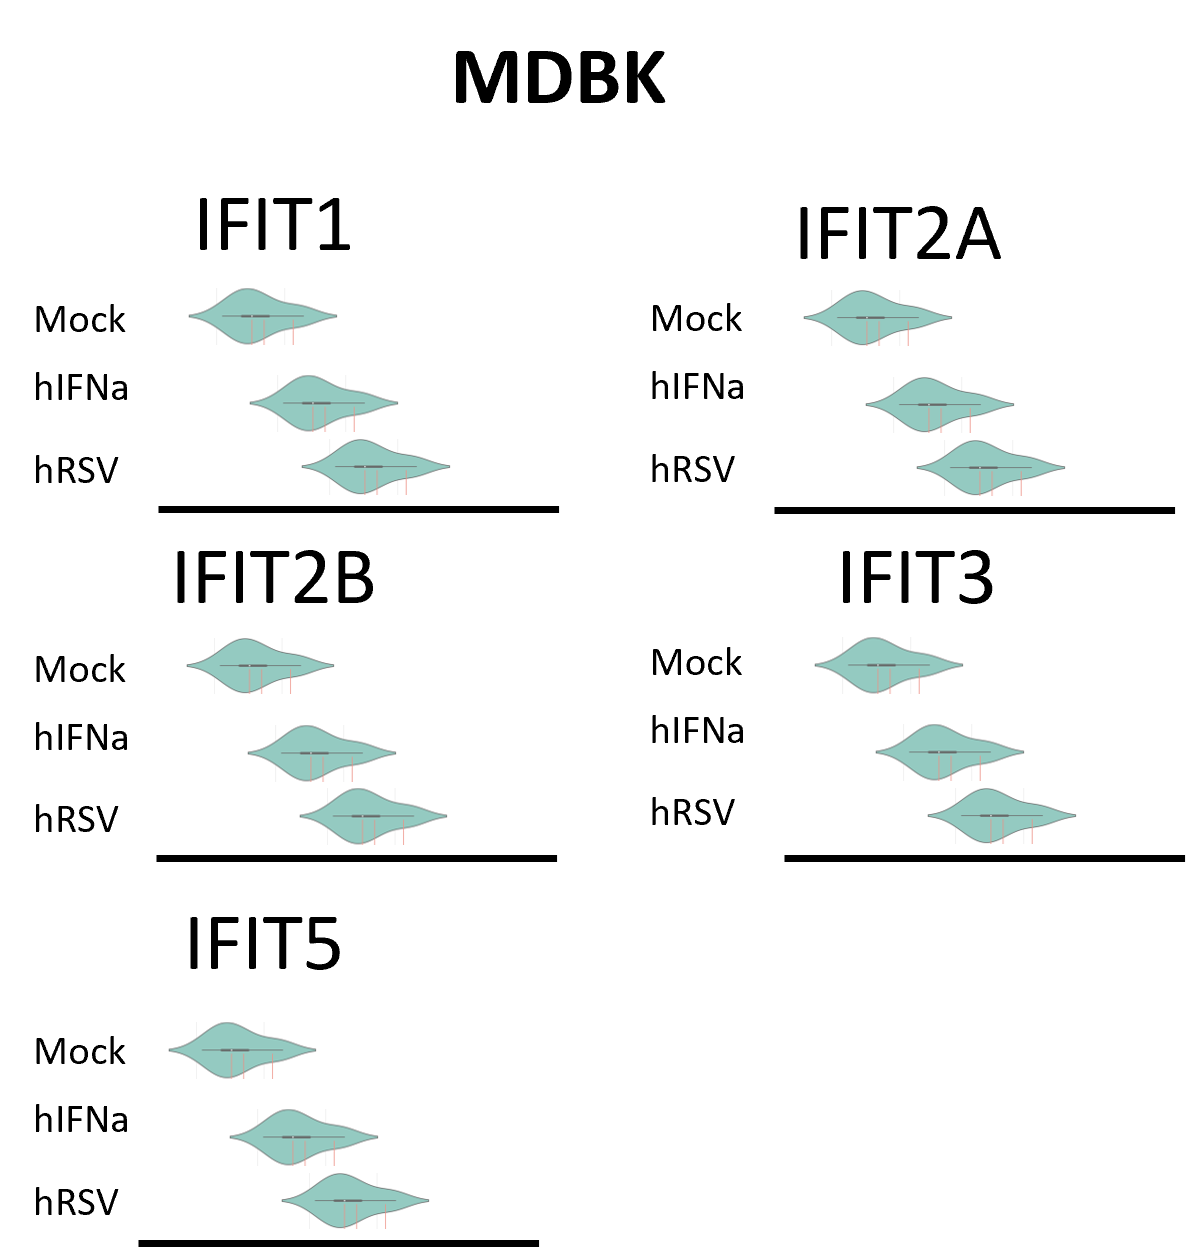
\includegraphics[width=1\linewidth]{09. Chapter 4/Figs/01. Localisation introduction/09. mdbk plots.png}
    \caption[Quantification Of Expression Changes of Bovine IFITs in MDBK Cells Subjected to bIFN\(\alpha\) or bRSV.]{\textbf{Quantification Of Expression Changes of Bovine IFITs in MDBK Cells Subjected to bIFN\(\alpha\) or bRSV.} Nascent bovine IFIT1 in the context of bRSV infection has been observed to localise with the respect of IB in three distinct spaces. We observed it either concentrated inside the central point of the IB structure, while having reduced signal on the inner IB edge, compared to the cytoplasm (top and bottom panels), being excluded from the IB structure (3rd panel), or colocalising on the inner edge of the IB structure while having reduced signal in the middle of the structure compared to cytoplasm, or the edge staining (2nd panel).}
    \label{fig:Quantification Of Expression Changes of Bovine IFITs in MDBK Cells Subjected to bIFN\(\alpha\) or bRSV}
\end{figure}

write about the potentially interesting things we see in infection and that further detailed analysis was conducted. Describe the definitions of different phenotypes. 